
\documentclass[submit]{ipsj}
%\documentclass{ipsj}

% \usepackage{graphicx}
\usepackage[dvipdfmx]{graphicx}
\usepackage{latexsym}

\def\Underline{\setbox0\hbox\bgroup\let\\\endUnderline}
\def\endUnderline{\vphantom{y}\egroup\smash{\underline{\box0}}\\}
\def\|{\verb|}

% \setcounter{巻数}{58}
% \setcounter{号数}{1}
% \setcounter{page}{1}


% \受付{2016}{3}{4}
% \再受付{2015}{7}{16}   %省略可能
% \再再受付{2015}{7}{20} %省略可能
% \再再受付{2015}{11}{20} %省略可能
% \採録{2016}{8}{1}


\begin{document}


% \title{ユーザの既訪問スポットの位置付けに基づく\\未訪問スポットの説明手法}
% \title{ユーザレビューを用いたスポット対応付け手法の\\提案とその応用}
\title{説明性向上のためのユーザレビューを用いた\\観光スポットの対応付け手法}

% \etitle{An Explanation Method of Unfamiliar Tourist Spots based on Roles of User's Familiar Spots}
% \etitle{Proposal of Spot Matching Method Using User Review And Its Application}
\etitle{An Association Method of Tourist Spots using User Reviews for Advancing Explainability}

% \affiliate{IPSJ}{情報処理学会\\
% IPSJ, Chiyoda, Tokyo 101--0062, Japan}

\affiliate{Uni}{工学院大学\\Kogakuin University,1--24--2,Nisisinjyuku,Tokyo 163--8677 Japan}

\author{潘 健太}{Kenta Han}{Uni}[em18011@ns.kogakuin.ac.jp]
\author{北山 大輔}{Daisuke Kitayama}{Uni}[kitayama@cc.kogakuin.ac.jp]

\begin{abstract}
近年,ユーザはWeb上の観光情報を活用して旅行計画を立てることが多くなっている.
しかし,旅行は未訪問スポットに行くことが多いため,観光情報を適切に入手することは困難である.
そこで,ユーザの未知なスポットに対する理解を支援するために,訪問したことがある観光スポットの特徴を用いて,未訪問エリアの観光スポットを説明する方法を提案する.
本研究では,まず,観光スポットのユーザレビューを用いて特徴ベクトルを作成する.
次に,ユーザにとっての観光スポットの位置付けを抽出するために,あるスポットに対し,既に訪れたスポットと比較した相対的特徴ベクトルを算出する.
最後に,相対的特徴ベクトル間の類似度に基づいて既訪問スポットと未訪問スポットを対応付けし,その対応関係を説明するための特徴語を抽出する.
また,プロトタイプシステムを構築し,既訪問スポットによる未訪問スポットの説明性の効果を評価する実験を行う.
\end{abstract}


\begin{jkeyword}
観光スポット,理解支援,ユーザレビュー,分散表現
\end{jkeyword}

\begin{eabstract}
% 多くの観光客は,レジャー旅行を計画するときに,オンラインから利用可能情報を得ている.しかし,旅行客は未訪問エリアに向けられるかもしれないので,この頼りはしばしば問題を生じそして誤解を招くようになる.
Most tourists resort to available information online when planning for leisure travel; however, this recourse often becomes problematic and misleading as tourist of the information may be directed to unfamiliar areas.
% この点に関して,我々は彼らが既に訪れたことがあるスポットの特徴を通して未訪問スポットを説明する方法を提案した.
On this regard, we proposed a method of explaining unfamiliar spots through the familiar features of spots they have visited.
% 本研究では,まず,観光スポットのユーザレビューを用いて特徴ベクトルを生成した.
In this paper, at first, we generated the feature vector using user reviews of the tourist spot.
% 次に,既に訪問したスポットと比較した相対的な特徴ベクトルを用いて,観光スポットの独特な特徴を抽出した.
Next, we used the relative feature vector compared with already visited spots to extract the role of the tourist spot for the user.
% 最後に,相対的特徴ベクトルの類似性によって訪問スポットを未訪問スポットと関連付け,さらにその関係を説明するキーワードを抽出した.
Finally, we associated the visited spot with the unfamiliar spot by the similarity of the relative feature vector, and further extracted keywords that explain the relation.
% また,システムのプロトタイプを開発し,既訪問スポットと未訪問スポットの間の説明情報の効果を評価した.
Furthermore, we developed a prototype of the system and evaluated the effect of the explanatory information between the familiar and unfamiliar spots.
\end{eabstract}

\begin{ekeyword}
tourist spots, explainability, tourist reviews, paragraph vector
\end{ekeyword}

\maketitle

%1
\section{はじめに}

旅行先を決定するとき,旅行者は観光スポット検索サイトや観光情報に関連する書籍を見て観光スポットを選び,旅行計画を立てる.
しかし,ユーザにとって訪問したいエリアは,訪問したことがなく不慣れであることが多い.
そのため,エリア内に数多く存在する観光スポットから,自身の要求に合う観光スポットを見つけることは容易ではない.

% Tripadvisor\footnote{https://www.tripadvisor.com/}やじゃらん\footnote{https://www.jalan.net/kankou/}などの観光スポット検索サイトでは,特定の観光スポットを訪問したことのあるユーザがレビューを投稿するため,観光スポットに関する豊富な情報が存在している.
% これらのレビューサイトは,ユーザの意思決定の材料になりえる.
ユーザの意識決定の材料の1つとして,Tripadvisor\footnote{https://www.tripadvisor.com/}やじゃらん\footnote{https://www.jalan.net/kankou/}などの観光スポット検索サイトがある.
これらのサイトには特定の観光スポットを訪問したことのあるユーザがレビューを投稿し,観光スポットに関する豊富な情報が存在している.
しかし,ユーザは検索エリアに関する事前知識がないため,どのスポットのレビューを読むべきか効率的に判断することは困難である.
そこで我々は,さまざまな観光スポットを効果的に理解するためには,ユーザが訪問した経験のあるスポットを使って未訪問スポットと類推できることが重要であると考えた.
たとえば,日本に初めて訪れるフランス人旅行者に対し,未訪問スポットである東京の「表参道」をパリにおける「シャンゼリゼ通り」と表現するとを理解しやすいであろう.
この考え方は,ユーザが以前に経験した物事を現在の物事に適用する一種の類推である.
既知の知識(ベースと呼ぶ)から概念(ターゲットと呼ぶ)を獲得するときに類推思考が働くとされる\cite{GENTNER1983155}.
構造の類似性には3種類あり,特徴の共有数で決まる「対象レベルの類似性」,ベースに存在する関係とターゲットに存在する関係の共有度に基づく「関係レベルの類似性」,および題の解法あるいは目標レベルでの類似性である「プラグマティックな類似性」とがある\cite{GENTNER1983155},\cite{Holyoak}.
本研究では,類推の質を明示的に扱うため,「関係レベルの類似性」に近いと考えられる.

本研究では,ユーザの未知なスポットに対する理解を支援するため,既に訪問したことがある観光スポットの特徴を用いて,未訪問エリアの観光スポットを説明する手法を提案する.
手法の詳細は3章で述べる.
図\ref{fig:Photo_Map}は,構築したプロトタイプシステムであり,訪問履歴として金閣寺等の京都のスポットを持つユーザが東京のエリアを検索した画面である.
未訪問エリアにある迎賓館に対して金閣寺が豪華絢爛という観点で類似する様子を示している.
このように,抽出したキーワードを提示することで,ユーザの未訪問スポットに対する理解の支援を目指す.

\begin{figure}[t]
  \begin{center}
    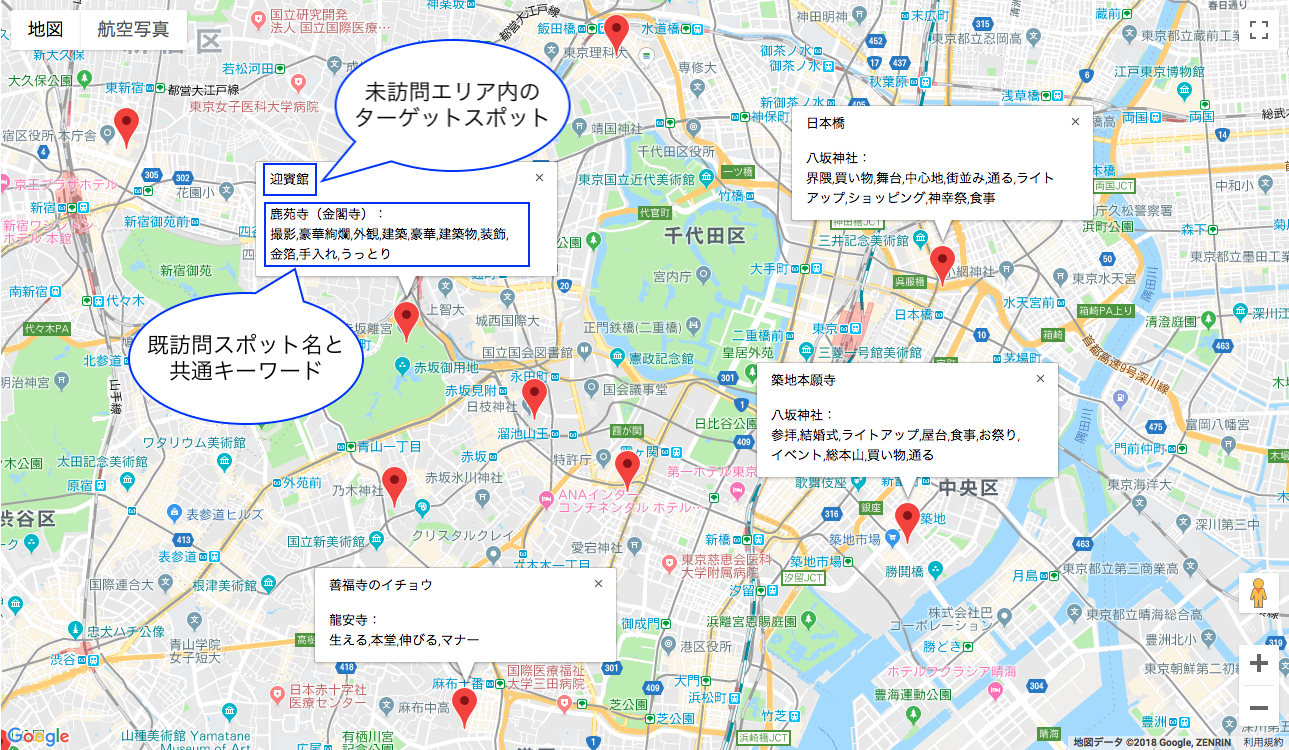
\includegraphics[clip,width=7.5cm]{picture/Photo_Map2_jap.png}
    \caption{プロトタイプシステム}
    \label{fig:Photo_Map}
   \end{center}
\end{figure}

%%%%%%%%%%%%%%%%%%%%%%%%%%%%%%%%%%%%%%%%%%
%%%%%%%%%%%%%%%%%%%%%%%%%%%%%%%%%%%%%%%%%
\section{関連研究}
ユーザの体験や履歴を利用した検索や推薦システムに関する研究は数多く発表されている.
倉島ら\cite{Kurashima}は,Flickrに投稿された写真のジオタグ情報を人々の旅行履歴として利用した旅行ルート推薦手法を提案した.
この手法では,ユーザの現在地から行きやすい場所とユーザの興味に合致した場所に移動しやすいと仮定し,行動モデルを生成している.
ユーザのジオタグ付き写真集合は,時間情報でソートすると個人の旅行履歴とみなすことができると考え,ジオタグ情報を利用してユーザの行動モデルを生成している.
北村ら\cite{Kitamura}は,一般的な物体認識を用いて,過去の個人旅行写真から推定したユーザの旅行の嗜好に基づき観光地を推薦する方法を提案した.
物体認識システムを用いて,写真で撮った被写体情報のキーワードを取得し,グラフ視覚化技術によってキーワードの共起を表現した.
また,グラフの視覚化技術に基づいて旅行写真付きのグラフを視覚化するユーザインターフェイスを紹介した.
Chengら\cite{Cheng}は,自由に利用できるコミュニティ投稿の写真を活用して,パーソナライズされた旅行のおすすめに焦点を当て,特定のユーザプロファイルまたは属性を考慮し,パーソナライズされた旅行の推奨を行うことを提案した.

観光地検索するとき,松本ら\cite{松本}はクチコミから特徴語を抽出して利用する研究を行った.抽出対象を任意の名詞として,4種類の手法,TFIDF,ATF(Average Term Frequency),ポアソン確率,エントロピーのうちどの手法が特徴語抽出に適しているのか検討を行った.また,抽出した特徴語を利用した検索支援システムを試作し,実験を通して特徴語提示の効果を検証した.
上原ら\cite{嶋田}はWebから観光情報を抽出し,複数の特徴ベクトルから観光地間の類似性を評価することで,観光地を推薦するシステムを提案した.観光地の特徴ベクトルは,知恵袋・ブログ上での共起キーワードと時系列分布,知恵袋上でのカテゴリ構造,観光地周辺施設,地図画像から生成した.これらの特徴ベクトルから観光地間の類似度の測定を行い,類似度の高い観光地を推薦した.
Kanazawaら\cite{Kanazawa}は印象語などの分析に基づき,行きたい場所のイメージから連想される行き先推薦システムを提案した.

このように,多くの研究はユーザに合致する観光地の抽出や,一般的な特徴の抽出に焦点をあてているが,本研究では,ユーザの選択性を高めるために,個人化した特徴を抽出する点で異なる.

%%%%%%%%%%%%%%%%%%%%%%%%%%%%%%%%%%%%%%%%%%
%%%%%%%%%%%%%%%%%%%%%%%%%%%%%%%%%%%%%%%%%%
\section{未訪問スポットと既訪問スポットの対応付け}
\label{sec:未訪問スポットと既訪問スポットの対応付け}

我々は,未訪問スポットを理解しやすくするために,最も位置付けの近いユーザの既訪問スポットを対応付ける手法を提案する.
まず,ユーザが既に訪問した複数個の観光スポットとこれから訪問したい観光スポットエリア情報を入力する.
本手法では,観光スポットのユーザレビューを用いて特徴ベクトルを生成する.
さらに,ユーザの観光地の位置付けを抽出するために,あるスポットに対し他の訪れたスポットと比較した相対的特徴ベクトルを算出する.
同様に,未訪問スポットもエリア内の各スポットの特徴ベクトルを求める.
また,未訪問エリアの各観光スポットの相対的特徴ベクトルを,そのエリアの他の観光スポットと比較して計算する.
次に,相対的特徴ベクトルの類似度によって既訪問スポットを未訪問スポットと対応付ける.
最後に,その関係性を説明するためのキーワードを抽出する.

%%%%%%%%%%%%%%%%%%%%%%%%%%%%%%%%%%%%%%%%%%
\subsection{スポットのユーザレビューを用いた相対的特徴ベクトル生成}
\label{subsec:スポットのレビューから相対的特徴ベクトル生成}
本稿では,2016年9月末までのじゃらんから得られたレビューデータを使用する.
分散表現\cite{Le}を用いて観光スポットの特徴ベクトルの作成する.
このとき,観光スポット毎のレビューをまとめて1つの文書として扱う.
本研究では,分散表現を計算するためにPythonのライブラリであるgensim\footnote{https://radimrehurek.com/gensim/models/doc2vec.html}を利用する.
学習方法として,Distributed Bag-of-Wordsを利用して,各スポットの全レビューを使って300次元で作成したベクトルを使う.
既訪問スポットや未訪問スポットのレビューベクトルは,形態素解析器であるMeCab\cite{Kudo}に辞書「mecab-ipadic-NEologd」\footnote{https://github.com/neologd/mecab-ipadic-neologd/}用いて,分かち書きし原型にしたレビューを利用して作成する.

各々の観光スポットは,ユーザによって,その強調するべき特徴は変化する.
たとえば,日本の有名な観光スポットを履歴に持つユーザにとっての「東京都庁舎展望台」と「金閣寺」について考える.
このとき,「金閣寺」の相対的特徴は,お寺,金色,京都などである.
「東京都庁舎展望台」の相対的特徴は,展望,夜景,建物,新宿などが考えられる.
% さまざまな観光スポットと比較すると,相対的特徴は一般的な特徴,カテゴリ,場所になる傾向がある.

一方,京都の寺院を履歴に持つユーザにとっての「金閣寺」と「清水寺」について考える.
このとき,同じ「金閣寺」でもお寺や京都などは特徴にはならず,「金閣寺」の相対的特徴は,金色,金箔,輝きなどとなる.
「清水寺」の相対的特徴は,舞台や一望などである.
% どちらも京都にある寺院であるため,京都や寺院に関連する特徴は相対的特徴にならない.
% その代わりに,より詳細な特徴が相対的特徴として得られる.

相対的特徴ベクトル$r_{state,i}$を,式\ref{math:Vector difference}として定義する.
\begin{equation}
  r_{state,i}=s_i-average(S_{state}-s_i)
  \label{math:Vector difference}
\end{equation}
相対的特徴ベクトルは,そのスポット自体の特徴ベクトルから他のスポットの特徴ベクトルの平均を引いた値によって得られる.
$S_{state} =\{s_1,s_2,\dots,s_n\}$は,既訪問スポット集合もしくは未訪問スポット集合である.
$state$が$f$であれば,既訪問スポット集合を意味し,$state$が$u$であれば,未訪問スポット集合を意味する.
$s_i$は集合$S_{state}$内の観光スポット$i$の特徴ベクトルを示している.

%%%%%%%%%%%%%%%%%%%%%%%%%%%%%%%%%%%%%%%%%%
\subsection{対応するスポットの決定と特徴語の抽出}
\label{subsec:対応するスポットの決定と特徴語の抽出}
未訪問エリア内のスポットを既訪問スポットと対応付ける.
% そのため,未訪問スポットと既訪問スポットを,それらの相対的特徴ベクトルの類似度に基づいて対応付けを行う.
% 関連付け手順について説明する.
具体的には,ある未訪問スポットの相対的特徴ベクトルに最も類似度が高い既訪問スポットを対応付ける.
類似度計算には,コサイン尺度を用いる.
ただし,類似度が閾値(本研究では0.125)以下である場合は対応付けを行わない.

スポットの対応関係を示すだけでは,どのような点で対応するのかを理解するのは難しい.
そこで,未訪問スポットと既訪問スポットの関係性を表すキーワードをユーザに提示する.
しかし,分散表現である相対的特徴ベクトルから単語の特徴を得ることはできないため,他の方法を用いて単語を抽出する.

すべてのレビューを\ref{subsec:スポットのレビューから相対的特徴ベクトル生成}節と同様に形態素解析器MeCabによって単語に分割する.
ただし,助詞,助動詞,連体詞,記号,ストップワードを削除している.

キーワード抽出手順について説明する.
まず,TFIDF法を使って対象となる既訪問スポットと未訪問スポットの特徴語とTFIDF値を求める.
IDF値を算出する集合は$S_{state}$を用いる.

2つのスポットに共通する特徴語のTFIDF値の調和平均を用いて,対応付けしたスポットの説明可能なキーワードとして抽出する.
各単語のスコアを式\ref{math:Harmonic Mean}によって定義する.
\begin{eqnarray}
  score(t,s_f,s_u) = \frac{2 \times tfidf(t,s_f) \times tfidf(t,s_u)}{tfidf(t,s_f) + tfidf(t,s_u)}
  \label{math:Harmonic Mean}
\end{eqnarray}
$tfidf(t,s_f)$と$tfidf(t,s_u)$は同じ単語に関する既訪問スポット$s_f$におけるTFIDF値と未訪問スポット$s_u$におけるTFIDF値を示している.
単語スコアの上位$N$個の単語を説明情報としてユーザに提示する.

\subsection{実行例}
\label{subsec:実行例}
\begin{table}[t]
  \caption{既訪問スポット集合と未訪問スポット集合}
  \label{table:既訪問スポット集合と未訪問スポット集合}
  \centering
  \begin{tabular}{l|l}
  \hline  \hline
  \multicolumn{1}{c|}{既訪問スポット名} & \multicolumn{1}{c}{未訪問スポット名} \\ \hline
  浅草寺                           & 東京ディズニーランド(R)                \\
  小田原城址公園                       & 新宿御苑                         \\
  伏見稲荷大社                        & 東京スカイツリー                     \\
  奈良公園                          & 東京タワー大展望台                    \\
  三島スカイウォーク                     & 明治神宮                         \\ \hline
  \end{tabular}
\end{table}

\begin{table*}[t]
  \caption{対応付け結果の例}
  \label{table:対応付け結果の例}
  \centering
  \begin{tabular}{l|l|l}
  \hline  \hline
  \multicolumn{1}{c|}{未訪問スポット} & \multicolumn{1}{c|}{既訪問スポット} & \multicolumn{1}{c}{特徴語}                     \\ \hline
  新宿御苑                      & 小田原城址公園                         & お花見,咲き誇る,園内,桜の時,のんびり,手入れ,自然,遊具,ツツジ          \\
  東京スカイツリー                     & 三島スカイウォーク                    & 富士山,揺れ,高所恐怖症,揺れる,天井,絶景,エレベーター,パノラマ,展望デッキ,昇る \\ \hline
  \end{tabular}
\end{table*}

表\ref{table:既訪問スポット集合と未訪問スポット集合}に示す,既訪問スポット集合と未訪問スポット集合を用いて対応付けを行った結果を説明する.
未訪問スポットは首都圏内を想定し5つのスポットを選んだ.
表\ref{table:対応付け結果の例}は,\ref{sec:未訪問スポットと既訪問スポットの対応付け}節で述べた提案手法を用いて抽出した対応付いたスポットの特徴語を示している.

未訪問スポット「新宿御苑」に対し,既訪問スポット「小田原城址公園」が対応付いた.
他に候補として「奈良公園」が考えられるが,「小田原城址公園」には花や遊具に対する記述が多く,「奈良公園」には鹿や草に対する記述が多い.
「新宿御苑」には花や遊具に対する記述が多いため,「小田原城址公園」と適切に対応付けたと考える.

未訪問スポット「東京スカイツリー」に対し「三島スカイウォーク」が対応づけられた.
どちらも眺めや高さに特徴があり関連付けられたと考えられる.
また,特徴語を見ると「富士山」が抽出されており,見える景色を想起させるような対応付けを行っていると考える.

%%%%%%%%%%%%%%%%%%%%%%%%%%%%%%%%%%%%%%%%%%
%%%%%%%%%%%%%%%%%%%%%%%%%%%%%%%%%%%%%%%%%%
\section{対応関係を表す特徴語抽出の評価}
\label{sec:対応関係を表す特徴語抽出の評価}
%%%%%%%%%%%%%%%%%%%%%%%%%%%%%%%%%%%%%%%%%%
\subsection{実験内容}
提案手法のうちの特徴語抽出部分について評価を行うため,他のキーワード抽出手法と比較して評価を行う.
以下の3つの方法を比較する.
\begin{itemize}
  \item 算術平均法
  \item 乗算法
  \item 提案手法(調和平均)
\end{itemize}

\begin{table}[t]
  \caption{対応関係を表す特徴語の実験結果}
  \label{table:対応関係を表す特徴語の実験結果}
  \centering
  \begin{tabular}{c|r|r|r}
  \hline \hline
  選択肢 & \multicolumn{1}{c|}{算術平均} & \multicolumn{1}{c|}{乗算} & \multicolumn{1}{c}{提案手法} \\ \hline
  1  & 28.28\%                  & 31.31\%                  & 29.29\%                 \\
  2  & 35.35\%                  & 31.31\%                  & 35.35\%                 \\
  3  & 10.10\%                   & 14.14\%                  & 12.12\%                 \\
  4  & 26.26\%                  & 23.23\%                  & 23.23\%                 \\ \hline
  \end{tabular}
\end{table}

% 方法Aと方法Bは,まず,各スポットの特徴として\ref{subsec:スポットのレビューから特徴ベクトル生成}節で作成された特徴ベクトルを使用する.
% そして,\ref{subsec:対応するスポットの決定と特徴語の抽出}節を用いて既訪問スポットと未訪問スポットの特徴語とTFIDF値を求める.

キーワードを抽出するとき,算術平均法では,2つのスポットに共通する特徴語のスコアとして算術平均を計算する.抽出した単語のスコアを式\ref{math:Mean}によって定義する.
\begin{eqnarray}
  score(t,s_f,s_u) = \frac{tfidf(t,s_f) + tfidf(t,s_u)}{2}
  \label{math:Mean}
\end{eqnarray}

乗算法では,2つのスポットに共通する特徴語のスコアとして乗算を計算する.抽出した単語のスコアを式\ref{math:Multi}によって定義する.
\begin{eqnarray}
  score(t,s_f,s_u) = tfidf(t,s_f) \times tfidf(t,s_u)
  \label{math:Multi}
\end{eqnarray}

% 式\ref{math:Mean},式\ref{math:Multi}の$TFIDF(t,d,f)$と$TFIDF(t,d,u)$は同じ単語に関する既訪問スポットのTFIDF値と未訪問スポットのTFIDF値を示している.単語スコアの上位$N$個の単語を説明情報としてユーザに提示する.

%%%%%%%%%%%%%%%%%%%%%%%%%%%%%%%%%%%%%%%%%%
\subsection{実験手順}
\label{subsec:実験手順}
クラウドソーシングのサービスである,CrowdWorks\footnote{https://crowdworks.jp/}を利用して23人の被験者を集めた.
% 各方法を用いて,被験者の既訪問スポットに基づいて,未訪問スポットの説明可能な情報を提示した.
まず,被験者は4から10個の自分が既に訪れたことのある観光スポットを入力した.
% 本実験では,入力文字列とシステム内のスポット名を照会するために,入力文字列から検索したスポット名候補の中から対象スポットを選択した.
次に,被験者は旅行などで行ったことがなく,これから訪れたい都道府県やエリアを入力した.

本実験では,それぞれの手法において,対応付けられた既訪問スポットと未訪問スポット,およびスポット同士の関係を説明する特徴語を最大で5つまで提示した.
結果を評価するために,被験者は以下の4つの選択肢から1つを選んだ.
\begin{enumerate}
  \item 2つのスポットには関係性があり,キーワード\footnote{関係を説明する特徴語のことであるが,被験者には単にキーワードと示した.}によって関係が明確になった.
  \item 2つのスポットの関係性があり,キーワードによって初めて気がついた.
  \item 2つのスポットには関係性があるが,キーワードは関係を表していない.
  \item 2つのスポットには関係性がない.
\end{enumerate}
%%%%%%%%%%%%%%%%%%%%%%%%%%%%%%%%%%%%%%%%%%
\subsection{実験結果と考察}
表\ref{table:対応関係を表す特徴語の実験結果}は,それぞれの手法における選択肢1から4それぞれの選択割合を示している.
乗算法では,多くの被験者が選択肢1を選択している.
このことから,乗算法は明らかな関係を表現する特徴語抽出ができることがわかった.
算術平均法と提案手法では,選択肢1の割合が減少し,選択肢2の割合が増加している.
このことから,算術平均法と提案手法は隠れた関係を表現する特徴語を見つけて被験者に提示することができると考えた.
しかし,算術平均法では,選択肢4の割合が増加しているため,提案手法より無関係な特徴語を抽出しやすくなったといえる.
また,選択肢1と2を合計すると,提案手法が最も高くなった.
このことから,スポットの関連を説明する特徴語抽出手法としては提案手法が妥当といえる.

%%%%%%%%%%%%%%%%%%%%%%%%%%%%%%%%%%%%%%%%%%
%%%%%%%%%%%%%%%%%%%%%%%%%%%%%%%%%%%%%%%%%%
\section{対応付けに関する評価}
\label{sec:対応付けに関する評価}
%%%%%%%%%%%%%%%%%%%%%%%%%%%%%%%%%%%%%%%%%%
\subsection{実験内容}
特徴語抽出については\ref{subsec:対応するスポットの決定と特徴語の抽出}節の手法を用いる.
提案手法のうちの対応付け部分について,以下の3つの手法を比較して評価を行う.
\begin{itemize}
  \item メタデータ法
  \item 分散表現法
  \item 提案手法
\end{itemize}

メタデータ法は,観光スポット検索サイトでスポットを検索するためのメタデータであるカテゴリ,滞在時間,訪問時期の一致を用いる.
まず,未訪問スポットに対し,すべてが一致する既訪問スポットを抽出する.
抽出できない場合は,季節,滞在時間,カテゴリの順に条件を緩和する.
既訪問スポットが複数ある場合は,レビュー数が最も多いスポットを選択する.
メタデータの例を以下に示す.
\begin{itemize}
 \item カテゴリ:神社・神宮・寺院,観光施設・名所巡り等
 \item 滞在時間:1時間未満,1--2時間等
 \item 訪問時期:1--12月,春,夏,秋,冬
\end{itemize}

分散表現法では,各スポットの特徴として\ref{subsec:スポットのレビューから相対的特徴ベクトル生成}節で作成した特徴ベクトルを使用する.
すなわち,式\ref{math:Vector difference}を用いずに,レビューから得た分散表現をそのまま用いる.

クラウドソーシングのサービスである,CrowdWorksを利用して24人の被験者を集めた.
実験手順は\ref{subsec:実験手順}節で説明した手順と同様である.

%%%%%%%%%%%%%%%%%%%%%%%%%%%%%%%%%%%%%%%%%%
\subsection{実験結果と考察}

\begin{table}[t]
  \caption{対応付けに関する実験結果}
  \label{table:対応付けに関する実験結果}
  \centering
  \begin{tabular}{c|r|r|r}
  \hline \hline
  選択肢 & \multicolumn{1}{c|}{メタデータ} & \multicolumn{1}{c|}{分散表現} & \multicolumn{1}{c}{提案手法} \\ \hline
  1  & 41.30\%                    & 33.85\%                    & 29.36\% \\
  2  & 43.48\%                    & 47.69\%                    & 48.62\% \\
  3  & 2.17\%                     & 2.31\%                     & 2.75\% \\
  4  & 13.04\%                    & 16.15\%                    & 19.27\% \\
  \hline
  対応付け数  & 46                    & 130                    & 109 \\
   \hline
  \end{tabular}
\end{table}

対応付けしたスポットの合計数は285である.
表\ref{table:対応付けに関する実験結果}は,それぞれの方法における選択肢1から5それぞれの選択割合を示している.
メタデータ法について,多くの被験者が選択肢2を選択している.
このことから,メタデータ法は明らかな関係にあるスポット同士を関連付けることができることがわかった.
他の方法と比較して,提案手法では,選択肢1の割合が減少し,選択肢2の割合が増加している.
このことから,提案手法は隠れた関係を見つけて被験者に提示することができると考えた.
しかし,選択肢4の割合も増加しているため,無関係なスポットを抽出しやすくなったといえる.

選択肢1と2を合計すると,メタデータ法が最も高くなる.
このことから,説明するためのスポットの対応付けの精度が最も高いといえる.
しかし,メタデータ法は対応付けすることができるスポットの数が他の手法に比べ半分以下であり,未訪問スポットの多くに説明を付与することができない.

分散表現法と提案手法を詳細に考察するために,既訪問スポットの入力別に分析した.
% 被験者が入力した既訪問スポットのカテゴリが異なる場合は同様の傾向を示した.
入力した既訪問スポットの半数以上が同一カテゴリのスポットであった被験者(表中の同じ場合)とそうではない被験者(表中の異なる場合)に分けて集計した.
表\ref{table:既訪問スポットのカテゴリの同異による評価割合}は選択肢1と選択肢2の評価の割合である.
提案手法を使用すると,カテゴリが異なる場合において,分散表現法よりも選択肢1および選択肢2の割合を増加させることができる.
相対的特徴ベクトルを用いることによって,カテゴリをこえて各スポットの特徴を求めることができるといえる.
% 既訪問スポットのジャンルが類似する場合では,方法Eの方がより良い評価となっている.
カテゴリが同じ場合の選択肢1は提案手法では,少なくなっている.
これは,相対的特徴ベクトルとしては,カテゴリの特徴が打ち消されたベクトルが生成されるため,明らかな関係となる対応付けが減ったと考えられる.
しかし,選択肢2が増えずに選択肢4が増え,無関係に見える対応付けを増やす結果となった.
そのため,入力スポットの種類によって対応付け手法を切り変えることが有効と考えられる.

\begin{table}[t]
  \caption{既訪問スポットのカテゴリの同異による評価割合}
  \label{table:既訪問スポットのカテゴリの同異による評価割合}
  \centering
  \begin{tabular}{c|c|r|r}
  \hline  \hline
                        & 選択肢 & \multicolumn{1}{c|}{分散表現} & \multicolumn{1}{c}{提案手法} \\ \hline
  異なる場合                 & 1   & 19.23\%                  & 21.10\%                 \\ \cline{2-4}
                        & 2   & 24.62\%                  & 25.69\%                 \\ \hline
  同じ場合                  & 1   & 14.62\%                  & 8.26\%                  \\ \cline{2-4}
  \multicolumn{1}{l|}{} & 2   & 23.08\%                  & 22.94\%                 \\ \hline
  \end{tabular}
\end{table}

%%%%%%%%%%%%%%%%%%%%%%%%%%%%%%%%%%%%%%%%%%
%%%%%%%%%%%%%%%%%%%%%%%%%%%%%%%%%%%%%%%%%%
\section{未訪問スポット説明の有効性評価}
\label{sec:未訪問スポット説明の有効性評価}
%%%%%%%%%%%%%%%%%%%%%%%%%%%%%%%%%%%%%%%%%%
\subsection{実験内容}
提案手法の有効性を評価するために以下の2つのシステムを使って比較する.
\begin{description}
  \item a.未訪問スポット名のみを表示
  \item b.未訪問スポット名,対応する入力スポット,対応を説明する特徴語を表示(提案手法)
\end{description}

被験者の入力は,これまでの実験と同様に,4個から10個の自分が既に訪れたことのある観光スポットと訪問したいエリアである.
ただし,エリアは2つ入力し,それぞれ別々にシステムa,システムbの入力として用いた.
なお,システムaとシステムbはランダムな順番で実行される.
システムを評価するために,被験者は以下の2つの設問について回答した.
また,それらの選択理由について自由記述で答えた.

\begin{description}
  \item Q1. 表示されたスポットの詳細情報はどちらの方が分かりやすいかを選択してください.
  \item Q2. 旅行の計画を立てる際にどちらの方が使いたいかを選択してください.
\end{description}

\subsection{実験結果と考察}
Q1に対する回答について,システムaとシステムbの結果はそれぞれ12件と38件となった.
被験者の回答理由の例を表\ref{table:システムaの方が良いと回答した被験者の自由記述}(システムa)および,表\ref{table:システムbの方が良いと回答した被験者の自由記述}(システムb)に示す.
また,
旅行の計画を立てる際にどちらの方が使いたいかに対する回答について,システムaとシステムbの結果はそれぞれ10件と40件となった.
被験者の回答より,得られた2つのシステムの特徴をまとめる.

システムbでは,キーワードや関連している情報が表示されており分かりやすいという特徴がある.
これに対し,システムaでは,スポット名のみが表示されているためシンプルで分かりやすいという特徴があるが,なぜそのスポットが検索されたのか分からないなどの否定的な回答も多数あった.
システムの表示情報が「シンプルな方が良い」と「詳細な情報が良い」の2つに大きく分けられているが,Q2の回答より80\%の被験者はシステムbの方が使いたいと回答しており,提案手法の方が評価が高いといえる.
また,システムbに関してスポットの写真を載せるとより分かりやすいなどの意見があり,画像による関連性の説明という拡張が考えられる.

\begin{table}[t]
  \caption{システムaの方が良いと回答した被験者の自由記述}
  \label{table:システムaの方が良いと回答した被験者の自由記述}
  \centering
  \begin{tabular}{l}
  \hline  \hline
  \begin{tabular}[c]{@{}l@{}}スポット名だけ書いてあるのでごちゃごちゃにならず、一目でどこに\\ 何があるか分かるからです.\end{tabular} \\ \hline
  スポットだけ表示されるところがシンプルで分かりやすかったから.                                                         \\ \hline
  シンプルにそのエリアの観光スポットを知ることが出来る.                                                             \\ \hline
  \end{tabular}
\end{table}

\begin{table}[t]
  \caption{システムbの方が良いと回答した被験者の自由記述}
  \label{table:システムbの方が良いと回答した被験者の自由記述}
  \centering
  \begin{tabular}{l}
  \hline  \hline
  自分が訪れた事のあるスポットと関連性があり連想しやすいから.                                                 \\ \hline
  \begin{tabular}[c]{@{}l@{}}どのような場所か想像しやすいので、計画を立てるのにも使いたい\\ と思ったから.\end{tabular} \\ \hline
  何と関連して表示された等詳細の情報が表示されわかりやすかった.                                                  \\ \hline
  \end{tabular}
\end{table}

%%%%%%%%%%%%%%%%%%%%%%%%%%%%%%%%%%%%%%%%%%
%%%%%%%%%%%%%%%%%%%%%%%%%%%%%%%%%%%%%%%%%%
\section{まとめと今後の課題}
\label{sec:まとめと今後の課題}

本研究では,ユーザが行きたい観光スポットが決まっていない場合に,ユーザの事前知識が不足しているため,観光検索サイトを使用してランキング,おすすめ情報やカテゴリなどを基に検索された観光スポットに対する理解が困難であることに着目した.
未訪問スポットに対する理解を支援するために,未訪問スポットをユーザが既に訪れたことがある既訪問スポットと比較することによって,理解を支援する説明手法を提案した.

キーワードの抽出の評価について,提案手法の方が既訪問スポットによる未訪問スポットの説明性が高いことを確認した.
対応付け手法の結果として,メタデータの一致に基づく手法では,未訪問スポットと対応付けできる既訪問スポットが最も少なくなることがわかった.
相対的特徴ベクトルと調和平均を利用することによって,各スポットの特徴を求めることができた.
また,未訪問スポットと既訪問スポットに対して意外性がある関連付けが可能で,ユーザが知らない観光スポットに対する興味と関心を集めることができる可能性があることを確認した.
システム評価について,提案手法の方がより詳細な情報を提示しているため,ユーザが未訪問スポットをイメージしやすいことを確認した.

今後の課題としては,レビュー数が少ないスポットに対する関連付けの精度が低いため,新たな方法を検討する必要がある.また,ある観光スポットに類似する特徴を持つ既訪問スポットで説明するだけではなく,既訪問スポット集合と対象観光スポットの関係を説明可能な可視化インタフェースへと拡張する予定である.

%%%%%%%%%%%%%%%%%%%%%%%%%%%%%%%%%%%%%%%%%%
\begin{acknowledgment}
本研究の一部は,2019科研費基盤研究(C)(課題番号:18K11551)によるものです.ここに記して謝意を表すものとします.
\end{acknowledgment}


%%%%%%%%%%%%%%%%%%%%%%%%%%%%%%%%%%%%%%%%%%
\begin{thebibliography}{11}
  \bibitem{Gentner}
    Gentner, D.:
      Structure-Mapping: A Theoretical Framework for Analogy,
      Cognitive Science, Vol.7, pp.155–170, 1983
  \bibitem{Holyoak}
    Holyoak, K.J. and Thagard, P.:
      Analogical Mapping by Constraint Satisfaction,
      Cognitive Science, Vol.13, pp.295–355, 1989
  \bibitem{Kurashima}
    Kurashima, T., Iwata, T., Irie, G. and Fujimura, K.:
      Travel route recommendation using geotags in photo sharing sites,
      CIKM '10 Proceedings of the 19th ACM international conference on Information and knowledge management, pp.579-588, 2010
  \bibitem{Kitamura}
    Kitamura, R. and Itoh, T.:
      Tourist Spot Recommmendation Applying Generic Object Recognition with Travel Photos,
      ITE Tech. Rep., Vol.42, No.12, AIT2018-94, pp.185-188, 2018
  \bibitem{Cheng}
    Cheng, A.J., Chen, Y.Y., Huang, Y.T. and Hsu, W.H.:
      Personalized Travel Recommendation by Mining People Attributes from Community-Contributed Photos,
      MM '11 Proceedings of the 19th ACM international conference on Multimedia, pp.83-92, 2011
  \bibitem{Le}
    Le, Quoc V. and Mikolov, T.:
      Distributed representations of sentences and documents,
      In Proceedings of the 31th International Conference on Machine Learning, ICML 2014, pp.1188–1196, 2014
  \bibitem{Kudo}
    Kudo, T., Yamamoto, K. and Matsumoto, Y.:
      Applying Conditional Random Fields to Japanese Morphological Analysis,
      Proceedings of the 2004 Conference on Empirical Methods in Natural Language Processing (EMNLP-2004), pp.230-237, 2004
  \bibitem{松本}
    松本 敦志, 杉本 徹:
      クチコミから抽出した特徴語を利用する観光地検索支援,
      第75回全国大会講演論文集, Vol.2013, No.1, pp.307-308, 2013
  % \bibitem{上原}
  %   上原 尚, 嶋田 和孝, 遠藤 勉,
  %     ``Web上に混在する観光情報を活用した観光地推薦システム'',
  %     社団法人 電子情報通信学会, 信学技報, Vol.112, No.367, pp.13-18, 2012
  \bibitem{嶋田}
    嶋田 和孝, 上原 尚, 遠藤 勉:
      集合知に基づく観光地推薦システムの構築,
      観光と情報:観光情報学会誌, Vol.10, No.1, pp.113-124, 2014
  \bibitem{Kanazawa}
    Kanazawa, Y., Hidaka, Y. and Ogawa, K.:
      Destination Retrieval System Using an Association Retrieval Method, International Journal of Future Computing and Comminication, Vol.2, No.3, pp.169-173, 2013.
  % \bibitem{Codd11}
  %   Y.T. Zheng, Z.J. Zha and T.S. Chua,
  %     ``Mining travel patterns from geotagged photos'',
  %     ACM Transaction on Intelligent System and Technology, Vol.3, No.3, pp.1-18, 2012

\end{thebibliography}

\begin{biography}
\profile{n}{潘 健太}{2018年工学院大学情報学部コンピュータ科学科卒業.
2018年同大学大学院工学研究科情報専攻修士課程入学,現在に至る.観光情報検索に興味を持つ.}
%
\profile{n}{北山 大輔}{2009年兵庫県立大学大学院環境人間学研究科博士後期課程修了.同年同学科客員研究員.2011同学科特任助教.2012年工学院大学情報学部助教.2016年同学部准教授,現在に至る.博士(環境人間学).Webマイニング,地理情報検索/推薦ベースを研究.電子情報通信学会.日本データベース学会各会員.}
\end{biography}

\end{document}
